%Copyright 2019 Christopher M. Jermaine (cmj4@rice.edu) and Risa B. Myers (rbm2@rice.edu)
%
%Licensed under the Apache License, Version 2.0 (the "License");
%you may not use this file except in compliance with the License.
%You may obtain a copy of the License at
%
%    https://www.apache.org/licenses/LICENSE-2.0
%
%Unless required by applicable law or agreed to in writing, software
%distributed under the License is distributed on an "AS IS" BASIS,
%WITHOUT WARRANTIES OR CONDITIONS OF ANY KIND, either express or implied.
%See the License for the specific language governing permissions and
%limitations under the License.
%===============================================================
\documentclass[aspectratio=169]{beamer}
\mode<presentation> 
{
\usetheme[noshadow, minimal,numbers,riceb,nonav]{Rice}
\usefonttheme[onlymath]{serif}
\setbeamercovered{transparent}
}
\useinnertheme{rectangles}

\usepackage[english]{babel}

\usepackage{mathptmx}
\usepackage{helvet}
\usepackage{courier}
\usepackage[T1]{fontenc}
\usepackage{trajan}
\usepackage{ textcomp }



\newcommand{\LIKES}{\textrm{LIKES}} 
\newcommand{\FREQUENTS}{\textrm{FREQUENTS}} 
\newcommand{\SERVES}{\textrm{SERVES}} 
\newcommand{\CAFE}{\textrm{CAFE}} 
\newcommand{\COFFEE}{\textrm{COFFEE}} 
\newcommand{\DRINKER}{\textrm{DRINKER}} 
\newcommand{\CB}{\textrm{\textquotesingle{Cold Brew}\textquotesingle}} 
\newcommand{\CBGOOD}{\textrm{COLDBREWGOOD}} 
\newcommand{\ALLPEEPS}{\textrm{ALLPEEPS}} 
\newcommand{\ALLCOMBOS}{\textrm{ALLCOMBOS}} 
\newcommand{\GOODCOFFEE}{\textrm{GOODCOFFEE}} 

\usepackage{listings}

\newenvironment{noindentitemize}
{ \begin{itemize}
 \setlength{\itemsep}{1.5ex}
  \setlength{\parsep}{0pt}   
  \setlength{\parskip}{0pt}
 \addtolength{\leftskip}{-2em}
 }
{ \end{itemize} }

\newenvironment{noindentitemize2}
{ \begin{itemize}
  \setlength{\itemsep}{0ex}
  \setlength{\parskip}{0pt}
  \setlength{\parsep}{0pt}   
  \addtolength{\leftskip}{-2em}  }
{ \end{itemize} }

\lstnewenvironment{SQL}
  {\lstset{
        aboveskip=5pt,
        belowskip=5pt,
        escapechar=!,
        mathescape=true,
        upquote=true,
        language=Python,
        basicstyle=\linespread{0.94}\ttfamily\footnotesize,
        morekeywords={PRINT, CURSOR, OPEN, FETCH, CLOSE, DECLARE, BEGIN, END, PROCEDURE, FOR, EACH, WITH, PARTITION, TEST, WHETHER, PROBABILITY, OUT,LOOP,IF,CONTINUE, HANDLER,CALL,FUNCTION, RETURNS, RETURN, BEFORE, ROW, OUT, 
        DELIMITER,CONCAT,FOUND,LEAVE, HANDLER, DOUBLE, TEMPORARY, REFERENCES },
        deletekeywords={VALUE, PRIOR},
        showstringspaces=true}
        \vspace{0pt}
        \noindent\minipage{0.47\textwidth}}
  {\endminipage\vspace{0pt}}
  

\setbeamerfont{block body}{size=\tiny}

%===============================================================%

\title[]
{Tools \& Models for Data Science}

\subtitle{Introduction to Python}

\author[]{Chris Jermaine \& Risa Myers}
\institute
{
  Rice University
}

\date[]{}

\subject{Beamer}


\begin{document}


\begin{frame}
 \titlepage
\end{frame}

%***********************************************************
\begin{frame}{Python}

\begin{itemize}
\item Old language, first appeared in 1991
	\begin{itemize}
	\item But updated often over the years
	\end{itemize}
\item Important characteristics
	\begin{itemize}
	\item Interpreted
	\item Dynamically-typed
	\item High level
	\item Multi-paradigm (imperative, functional, OO) 
	\item Generally compact, readable, easy-to-use
	\end{itemize}
\item Boom in popularity last five years
	\begin{itemize}
\item Now the first programming language learned in many CS departments
	\end{itemize}
\end{itemize}
\end{frame}

%***********************************************************
\begin{frame}{Python: Why So Popular for Data Science?}

\begin{itemize}
\item Dynamic typing/interpreted
	\begin{itemize}
\item 	Type a command, get a result
\item 	No need for compile/execute/debug cycle
	\end{itemize}
\item Quite high-level: easy for non-CS people to pick up
	\begin{itemize}
\item 	Statisticians, mathematicians, physicists...
	\end{itemize}
\item More of a general-purpose programming language than R
	\begin{itemize}
\item 	More reasonable target for larger applications
\item 	More reasonable as API for platforms such as Spark
	\end{itemize}
\item Can be used as lightweight wrapper on efficient numerical codes
% can encapsulate code written in C++
	\begin{itemize}
\item 	Unlike Java, for example
	\end{itemize}
\end{itemize}
\end{frame}

%***********************************************************
\begin{frame}[fragile]{Python Basics}

\begin{itemize}
\item Since Python is interpreted, can just fire up Python shell, ipython, or a Jupyter Notebook
	\begin{itemize}
	\item Then start typing
	\end{itemize}
\item A first Python program
\end{itemize}
\begin{SQL}
def Factorial (n):
     if n == 1 or n == 0:
          return 1
     else:
          return n * Factorial (n - 1)

Factorial (12)
\end{SQL}
\end{frame}


%***********************************************************
\begin{frame}{Python Basics Continued}

\begin{itemize}
\item Spacing and indentation
        \begin{itemize}
        \item Indentation is important
	\item No begin/end nor \{\}
	\item Indentation signals code block
        \end{itemize}
\item Variables
        \begin{itemize}
        \item No declaration
	\item All type checking is dynamic
	\item Just use them
        \end{itemize}
\end{itemize}
\end{frame}

%***********************************************************
\begin{frame}{Python Basics Continued}

\begin{itemize}
\item Dictionaries
        \begin{itemize}
        \item Standard container type is dictionary/map
        \item Example: $\texttt{wordsInDoc = \{\}}$ creates an empty dictionary
	\end{itemize}
\item Adding Data
        \begin{itemize}
	\item Add data by saying $\texttt{wordsInDoc[23] = 16}$
	\item Now can write something like $\texttt{if wordsInDoc[23] == 16:}$ ...
	\item What if $\texttt{wordsInDoc[23]}$ is not there? Will crash
	\item Protect with $\texttt{wordsInDoc.get(23, 0) \ldots}$ returns 0 if key 23 not defined
	\end{itemize}
\end{itemize}
\end{frame}

%***********************************************************
\begin{frame}[fragile]{Encapsulation}

\begin{itemize}
\item Functions/Procedures
        \begin{itemize}
	\item Defined using $\texttt{def myFunc (arg1, arg2):}$
	\item Make sure to indent!
	\item Procedure: no return statement
	\item Function: return statement
        \end{itemize}
\item Remember:
        \begin{itemize}
        \item No marker to end function or procedure
        \item It ends when you stop indenting
        \end{itemize}
\end{itemize}

\begin{SQL}
def Factorial (n):
     if n == 1 or n == 0:
          return 1
     else:
          return n * Factorial (n - 1)

Factorial (12)
\end{SQL}

\end{frame}

%***********************************************************
\begin{frame}{Loops}

\begin{itemize}
\item Several common forms
\item Looping through a range of values
        \begin{itemize}
	\item Of form  $\texttt{for var in range (0, 50)}$
	\item Loops for $\texttt{var}$ in $\texttt{\{0, 1, ..., 49\}}$
        \end{itemize}
\item Looping through data structures
        \begin{itemize}
        \item Example: $\texttt{for var in dataStruct}$
	\item loops through each entry in $\texttt{dataStruct}$
	\item $\texttt{dataStruct}$ can be an array, or a dictionary 
	\item If array, you loop through the entries
	\item If dictionary, you loop through the keys
        \end{itemize}
\end{itemize}
\end{frame}

%***********************************************************
\begin{frame}[fragile]{Loops Continued}

\begin{itemize}
\item An example
\end{itemize}
\begin{SQL}
a = {}
a[1] = 'this'
a[2] = 'that'
a[3] = 'other'
for b in a:
   print(a[b])

this
that
other
\end{SQL}
\end{frame}

 
%***********************************************************
\begin{frame}{NumPy}

\begin{itemize}
\item NumPy is a Python package
\item Most important one for data science!
	\begin{itemize}
	\item Can use it to do super-fast math, statistics
	\item Most basic type is NumPy array
	\item Used to store vectors, matrices, tensors
	\end{itemize}
\item You will get some reasonable experience with NumPy
\item Load with $\texttt{import numpy as np}$
\end{itemize}
\end{frame}

%***********************************************************
\begin{frame}{NumPy Arrays: What Are They?}

\begin{itemize}
\item Multi-dimensional array data structure
\item And associated API
\item Widely used for data intensive programming...
 \begin{itemize}
 \item Linear algebra
 \item Data science
 \item Machine Learning
 \end{itemize}
\end{itemize}
\end{frame}

%***********************************************************
\begin{frame}[fragile]{NumPy Arrays: Your Best Friend In DS}

\begin{itemize}
\item Writing control flow code in DS programming is BAD
        \begin{itemize}
	\item Kind of like in SQL
        \end{itemize}
\item Python is interpreted
        \begin{itemize}
	\item Time for each statement execution generally large
	\item And in DS, you have a lot of data
	\item So this code can take a long time:
        \end{itemize}
\begin{SQL}
for b in range(0, BIG):
   a[b] = b
 
sum = 0
for b in a:
   sum += a[b]
\end{SQL}

\item Fewer statements executed, even if the work is the same...
	\begin{itemize}
	\item ...means better performance!
	\end{itemize}
\end{itemize}
\end{frame}

%***********************************************************
\begin{frame}{To Reduce Number of Statements...}

\begin{itemize}
\item Use NumPy arrays where possible
\item Goal: one line of Python to process entire array!
\item Some guidelines:
	\begin{itemize}
	\item Try to replace dictionaries with NumPy arrays
	\item Try to replace loops with bulk array operations
	\begin{itemize}
	\item Backed by efficient, low-level implementations
	\end{itemize}
	\item This is known as ``vectorized'' programming
	\end{itemize}
\end{itemize}
\end{frame}

%***********************************************************
\begin{frame}[fragile]{Creating and Filling NumPy Arrays}

\begin{itemize}
\item To create a 2 by 5 array, filled with 3.14

\begin{SQL}
>>> np.full((2, 5), 3.14)

array([[ 3.14, 3.14, 3.14, 3.14, 3.14],
       [ 3.14, 3.14, 3.14, 3.14, 3.14]])
\end{SQL}

\item To create a 2 by 5 array, filled with 0

\begin{SQL}
>>> np.zeros((2, 5))

array([[ 0., 0., 0., 0., 0.],
       [ 0., 0., 0., 0., 0.]])
\end{SQL}
\end{itemize}
\end{frame}

%***********************************************************
\begin{frame}[fragile]{1D Numpy Arrays vs. Python Lists}

\begin{itemize}
\item Just like Python lists
\item Create an array from a range

\begin{SQL}
>>> a = np.arange(1, 11, 2)
array([1, 3, 5, 7, 9])
>>> l = list(range(1, 11, 2))
[1, 3, 5, 7, 9]
\end{SQL}


\end{itemize}
\end{frame}
%***********************************************************
\begin{frame}[fragile]{Accessing Elements}

\begin{itemize}
\item Just like Python lists

\begin{SQL}
>>> a[0]
1
>>> l[0]
1
>>> a[3:]
array([7, 9])
>>> l[3:]
[7,9]
\end{SQL}


\end{itemize}
\end{frame}



%***********************************************************
\begin{frame}[fragile]{Other Useful Numpy Functions}

\begin{itemize}
\item sqrt -- return an array with the square root of each member of the array
\begin{SQL}
np.sqrt(a)
\end{SQL}
\item square -- return an array with the square of each member of the array
\begin{SQL}
np.square(a)
\end{SQL}
\item sum - return the sum of the values in the array
\begin{SQL}
a.sum()
\end{SQL}
\end{itemize}
\end{frame}

%***********************************************************

\begin{frame}{Pause Here Until Later}
\begin{enumerate}
\item Python review
\item Introduction to numpy arrays
\end{enumerate}

\begin{itemize}
	\item[?] How can we use what we learned today?
	\vspace{2em}
	\item[?] What do we know now that we didn't know before?
\end{itemize}
\end{frame}


%***********************************************************
\begin{frame}[fragile]{More Complicated Creation Examples}

\begin{itemize}
\item To create an array with odd numbers thru 10
\end{itemize}
\begin{SQL}
>>> np.arange(1, 11, 2)

array([1, 3, 5, 7, 9])
\end{SQL}

\begin{itemize}
\item To ``tile'' an array 
\end{itemize}
\begin{SQL}
>>> np.tile (np.arange(1, 11, 2), (1, 2))

array([[1, 3, 5, 7, 9, 1, 3, 5, 7, 9]])

>>> np.tile (np.arange(1, 11, 2), (2, 1))

array([[1, 3, 5, 7, 9],
       [1, 3, 5, 7, 9]])
\end{SQL}
\end{frame}

%***********************************************************
\begin{frame}[fragile]{Accessing Subparts of Arrays}

\begin{columns}
\begin{column}{0.5\textwidth}	


\begin{itemize}
\item First we create a 2-d array (matrix)

\begin{SQL}
>>> a1 = np.arange(1, 6, 1)
>>> a2 = np.arange(2, 7, 1)
>>> a3 = np.arange(3, 8, 1)
>>> a = np.row_stack ((a1, a2, a3))
>>> a

array([[1, 2, 3, 4, 5],
       [2, 3, 4, 5, 6],
       [3, 4, 5, 6, 7]])
\end{SQL}

\end{itemize}
\end{column}

\begin{column}{0.5\textwidth}
{\centering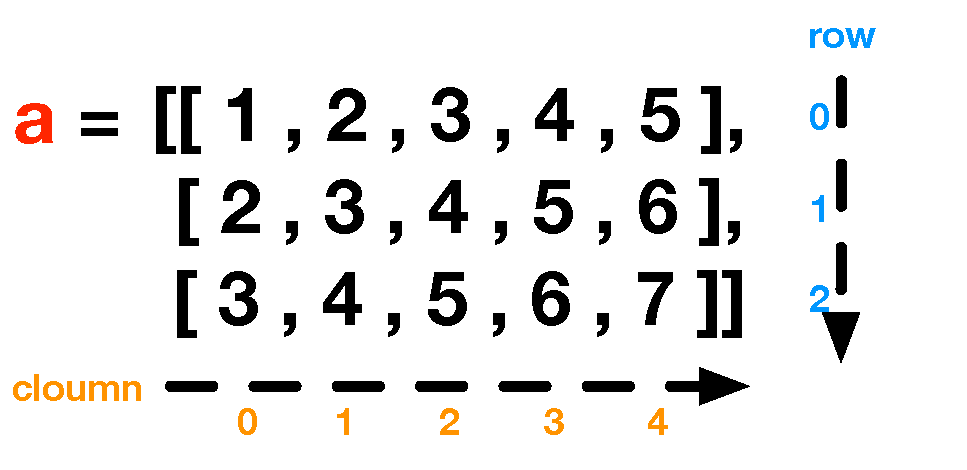
\includegraphics[width=1\textwidth]{./lectPython/Canvas02.pdf}\par}	
\end{column}

\end{columns}
\end{frame}

%***********************************************************
\begin{frame}[fragile]{Accessing Subparts of Arrays (cont)}

\begin{SQL}
array([[1, 2, 3, 4, 5],
       [2, 3, 4, 5, 6],
       [3, 4, 5, 6, 7]])
\end{SQL}

\begin{itemize}
\item Say we want first two rows:

\begin{SQL}
>>> a[1:,]
\end{SQL}

\item[?] Will this work?
\end{itemize}

\end{frame}
%***********************************************************
\begin{frame}[fragile]{Accessing Subparts of Arrays (cont)}

\begin{columns}
\begin{column}{0.5\textwidth}	
\begin{SQL}
array([[1, 2, 3, 4, 5],
       [2, 3, 4, 5, 6],
       [3, 4, 5, 6, 7]])

>>> a[1:,]

array([[2, 3, 4, 5, 6],
       [3, 4, 5, 6, 7]])

>>> a[1:]
array([[2, 3, 4, 5, 6],
       [3, 4, 5, 6, 7]])
\end{SQL}

\begin{itemize}
\item Indices start with 0
\item Gets rows 1, 2, 3, and so on
\end{itemize}
\end{column}

\begin{column}{0.5\textwidth}
{\centering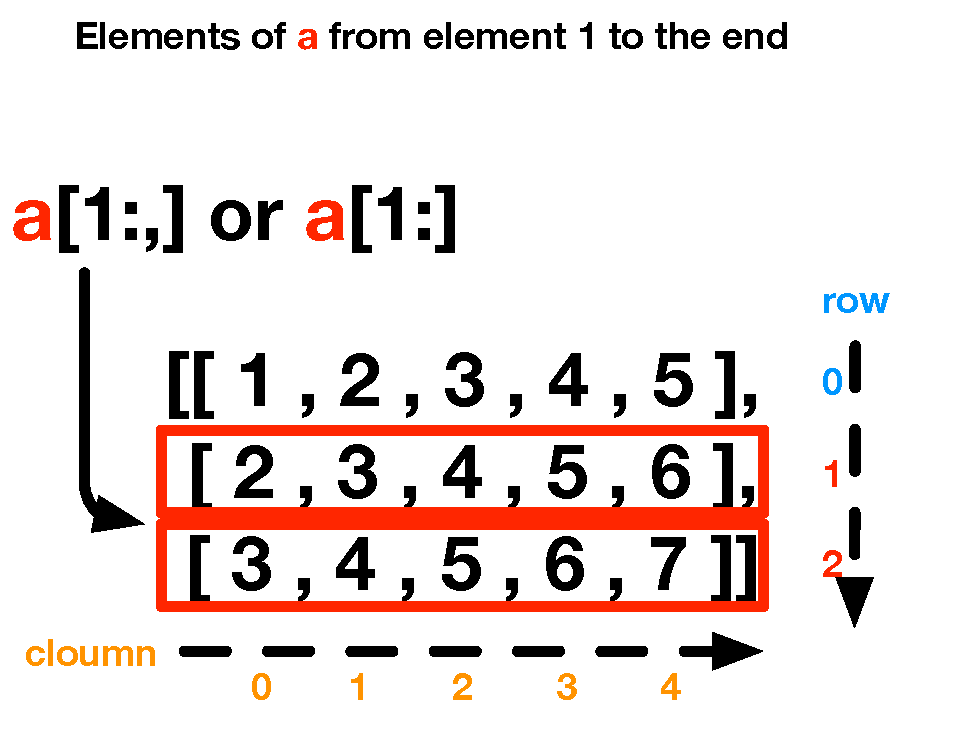
\includegraphics[width=1\textwidth]{./lectPython/Canvas04.pdf}\par}	
\end{column}

\end{columns}
\end{frame}

%***********************************************************
\begin{frame}[fragile]{Accessing Subparts of Arrays (cont)}

\begin{columns}
\begin{column}{0.5\textwidth}
\begin{itemize}
\item Say we want the last row:

\begin{SQL}
>>> a[2:3,]
array([[3, 4, 5, 6, 7]])

>>> a[2:3]
array([[3, 4, 5, 6, 7]])

\end{SQL}

\item Note: still a 2-d array.  Want a vector?

\begin{SQL}
>>> a[2:3][0]

array([3, 4, 5, 6, 7])
\end{SQL}
\end{itemize}
\end{column}

\begin{column}{0.5\textwidth}
{\centering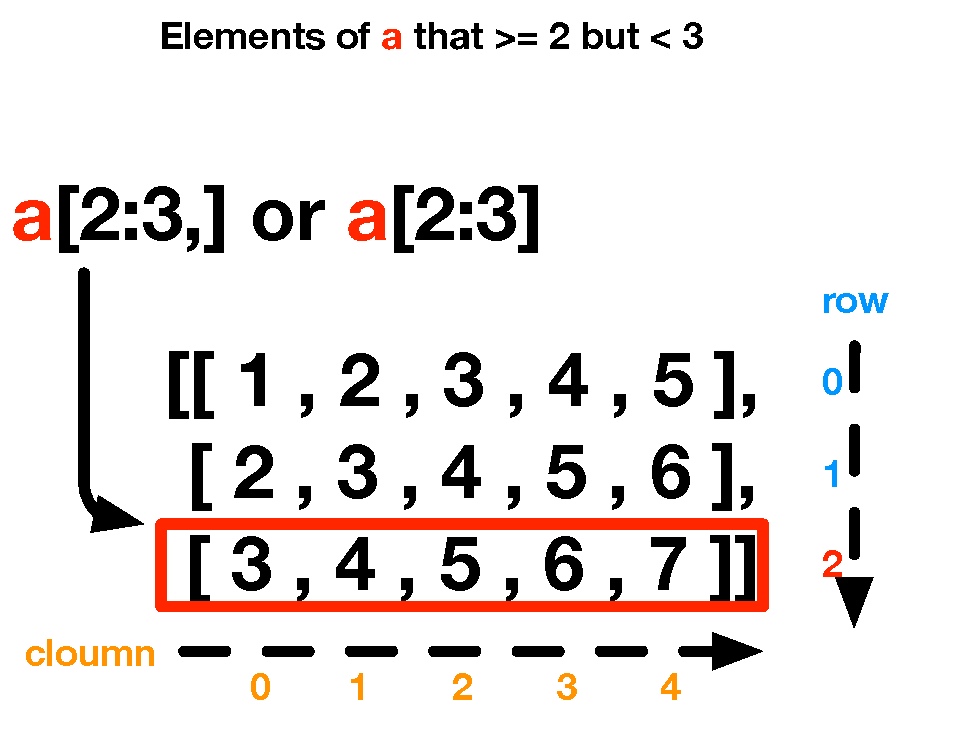
\includegraphics[width=1\textwidth]{./lectPython/Canvas05.pdf}\par}	
\end{column}

\end{columns}
\end{frame}

%***********************************************************
\begin{frame}[fragile]{Accessing Subparts of Arrays (cont)}

\begin{columns}
\begin{column}{0.5\textwidth}
\begin{itemize}
\item Now we want the second, third columns:

\begin{SQL}
>>> a[:,1:3]

array([[2, 3],
       [3, 4],
       [4, 5]])

>>> a[:,np.array((1,2))]

array([[2, 3],
       [3, 4],
       [4, 5]])

\end{SQL}
\end{itemize}
\end{column}

\begin{column}{0.5\textwidth}
{\centering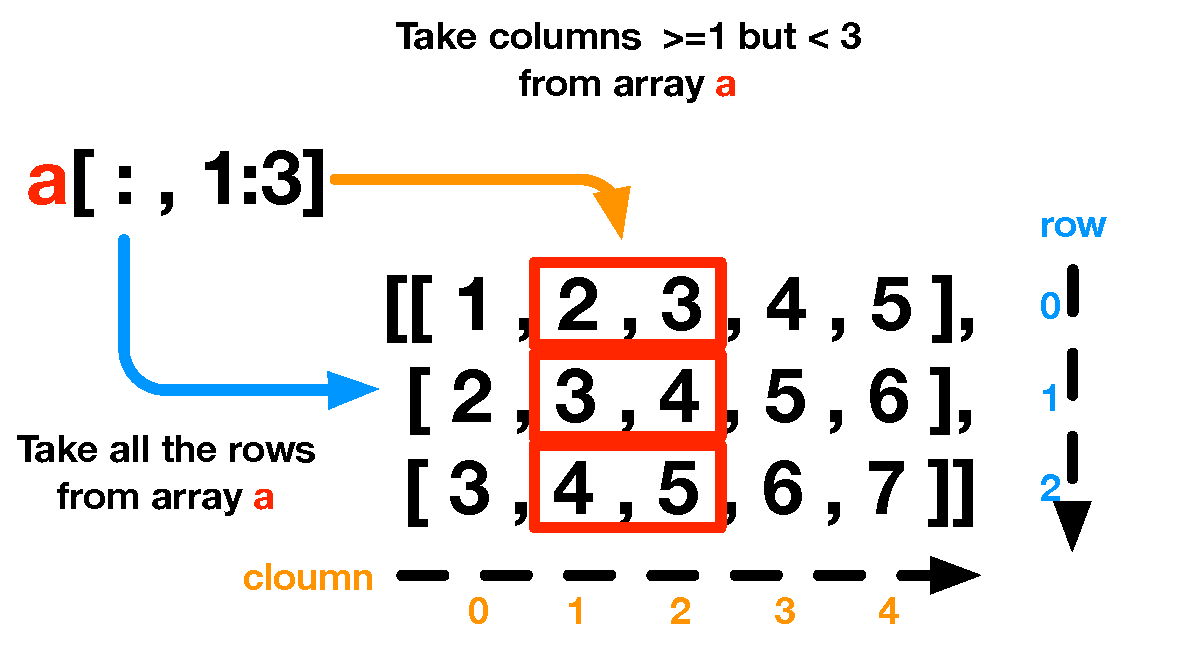
\includegraphics[width=1\textwidth]{./lectPython/Canvas01.pdf}\par}	
\end{column}

\end{columns}
\end{frame}

%***********************************************************

\begin{frame}[fragile]{Aggregations Over Arrays}

\begin{itemize}
\item In statistical/data analytics programming...
	\begin{itemize}
	\item Tabulations: max, min, etc. over NumPy arrays are ubiquitous
	\end{itemize}
\item Key operation allowing this is sum

\begin{SQL}
>>> a = np.arange(1, 6, 1)
>>> a

array([1, 2, 3, 4, 5])

>>> a.sum ()

15
\end{SQL}
\end{itemize}
\end{frame}

%***********************************************************

\begin{frame}[fragile]{Aggregations Over Arrays (cont)}

\begin{columns}

\begin{column}{0.5\textwidth}
\begin{itemize}
\item Can sum along dimension(s) of higher-d array 

\begin{SQL}
>>> a

array([[1, 2, 3, 4, 5],
       [2, 3, 4, 5, 6],
       [3, 4, 5, 6, 7]])

>>> a.sum (0)

array([6, 9, 12, 15, 18])

>>> a.sum (1)

array([15, 20, 25])
\end{SQL}
\item Think about sum collapsing the array along the specified axis
\end{itemize}
\end{column}

\begin{column}{0.5\textwidth}
%\begin{itemize}
	{\centering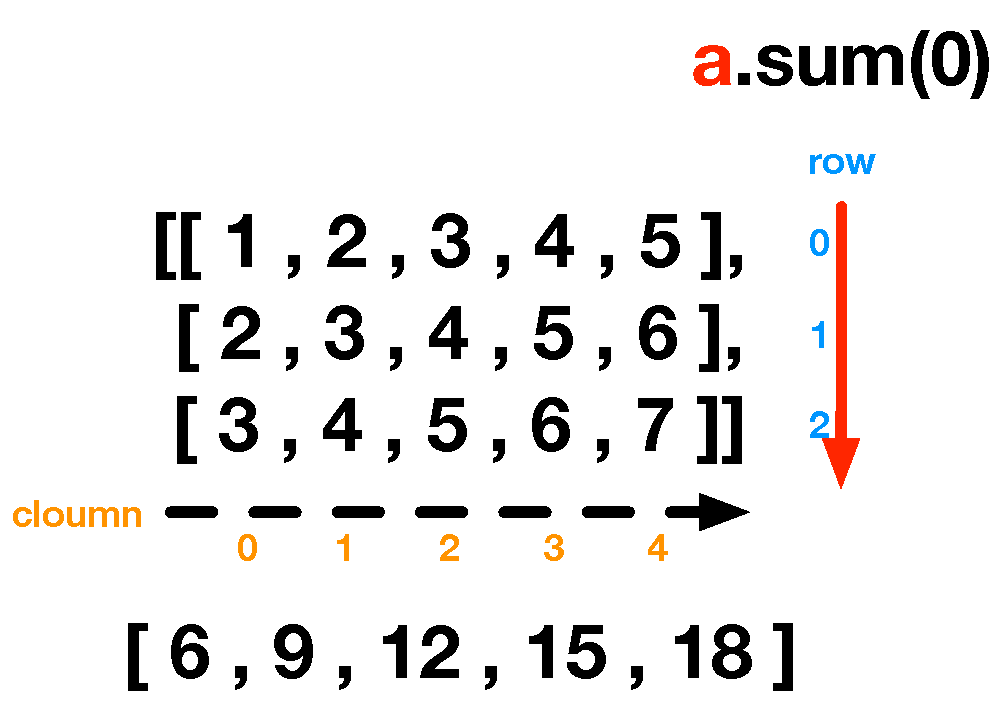
\includegraphics[width=0.9\textwidth]{./lectPython/Canvas07.pdf}\par}
	{\centering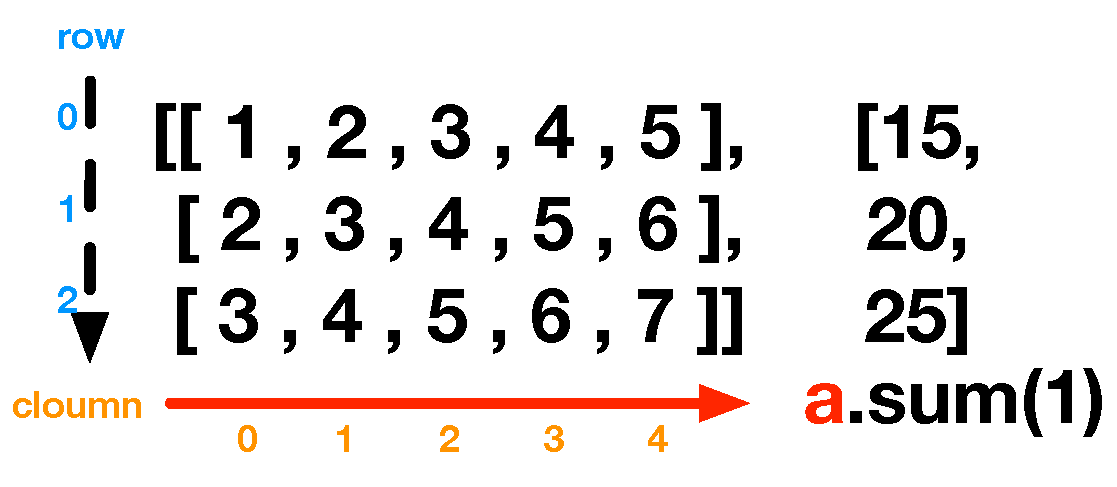
\includegraphics[width=0.9\textwidth]{./lectPython/Canvas08.pdf}\par}
%\end{itemize}}
	
\end{column}

\end{columns}
\end{frame}

%***********************************************************
\begin{frame}[fragile]{Aggregations Over Arrays (cont)}

\begin{itemize}
\item Can find the maximum the same way

\begin{SQL}
>>> a
array([[10, 2,  3, 4, 5],
       [ 2, 3, 13, 5, 6],
       [ 3, 4,  5, 6, 7]])

>>> a.max ()

13

>>> a.max (0)

array([10, 4, 13, 6, 7])

>>> a.max (1)

array([10, 13, 7])
\end{SQL}
\end{itemize}
\end{frame}

%***********************************************************
\begin{frame}[fragile]{Aggregations Over Arrays (cont)}

\begin{itemize}
\item Can find the position of the max as well

\begin{SQL}
>>> a

array([[10, 2,  3, 4, 5],
       [ 2, 3, 13, 5, 6],
       [ 3, 4,  5, 6, 7]])

>>> a.argmax ()

7

>>> a.argmax (1)

array([0, 2, 4])
\end{SQL}
\end{itemize}
\end{frame}
% argmax(0) is by column
% argmax(1) is by row

%***********************************************************
\begin{frame}[fragile]{Shape}

\begin{itemize}
\item Get a tuple of array dimensions

\begin{SQL}
>>> a

array([[10, 2,  3, 4, 5],
       [ 2, 3, 13, 5, 6],
       [ 3, 4,  5, 6, 7]])

>>> a.shape

(3, 5)
\end{SQL}
\end{itemize}
\end{frame}


%***********************************************************
%
%\begin{frame}{Now We Need a ``Real Life'' Set of Problems}
%
%\begin{noindentitemize}
%\item ...where we can apply some of these ideas
%\end{noindentitemize}
%\end{frame}
%
%%***********************************************************
%
%\begin{frame}{Latent Dirichlet Allocation (LDA)}
%
%\begin{noindentitemize}
%\item We will use data created by a statistical model called ``LDA''
%\item LDA: stochastic model for generating a document corpus
%\item Most widely-used ``topic model''
%\item A ``topic'' is a set of words that appear together with high prob
%	\begin{noindentitemize2}
%	\item Intuitively: set of words that all have to do with the same subject
%	\end{noindentitemize2}
%\end{noindentitemize}
%\end{frame}
%
%%***********************************************************
%
%\begin{frame}{LDA Typically Used To Analyze Text}
%
%\begin{noindentitemize}
%\item Idea
%	\begin{noindentitemize2}
%	\item If you can analyze a corpus...
%	\item And figure out a set of $k$ topics...
%	\item As well as how prevalent each topic is in each document
%	\item You then know a lot about the corpus
%	\item Ex: can use this prevalence info to search the corpus
%	\item Two docs have similar topic compositions? Then they are similar!
%	\end{noindentitemize2}
%\end{noindentitemize}
%\end{frame}
%
%%***********************************************************
%
%\begin{frame}{Forward vs. Backward modeling}
%
%\begin{noindentitemize}
%\item Often, we want to ``learn'' an LDA model from an existing corpus
%	\begin{noindentitemize2}
%	\item That is, you have a real data set
%	\item And you analyze the the data set
%	\item Goal: figure out how LDA model could have produced it
%	\item This is ``backward'' modeling
%	\end{noindentitemize2}
%\item But can also use it to generate a corpus
%	\begin{noindentitemize2}
%	\item ``Forward'' modeling using LDA far less common
%	\item But we'll use the forward LDA process to generate our lab data
%	\end{noindentitemize2}
%\end{noindentitemize}
%\end{frame}
%
%%***********************************************************
%
%\begin{frame}{Dictionary Models}
%
%\begin{noindentitemize}
%\item LDA is a ``Bag of Words'' model
%\item Does not impose ordering on words in doc
%\item Uses a dictionary
%	\begin{noindentitemize2}
%        \item Dictionary is a map from each of $m$ unique words in corpus
%        \item To a number from $\{1...m\}$
%	\end{noindentitemize2}
%\item Example:
%	\begin{noindentitemize2}
%	\item Dictionary might be: (0, bad) (1, I) (2, can't) (3, stand)
%(4, COMP101), (5, to) (6, leave) (7, love) (8, beer) (9, humanities) (10, classes)
%	\end{noindentitemize2}
%\end{noindentitemize}
%\end{frame}
%
%%***********************************************************
%
%\begin{frame}{From Dictionary to Bag of Words}
%
%\begin{noindentitemize}
%\item Document is a vector $x$
%	\begin{noindentitemize2}
%	\item $x[i]$ ($i$th entry in vector) is number of times dictionary word $i$ appears in doc
%	\end{noindentitemize2}
%\item Recall our dictionary is (0, bad) (1, I) (2, can't) (3, stand)
%(4, COMP101), (5, to) (6, leave) (7, love) (8, beer) (9, humanities) (10, classes)
%\item Then
%	\begin{noindentitemize2}
%	\item Sentence ``I can't stand bad beer'' is $\langle 1,1,1,1,0,0,0,0,1,0,0 \rangle$
%	\item Sentence ``I love beer I can't love humanities classes'' is $\langle 0,2,1,0,0,0,0,2,1,1,1 \rangle$
%	\end{noindentitemize2}
%\end{noindentitemize}
%\end{frame}
%
%%***********************************************************
%
%\begin{frame}{LDA Step One}
%
%\begin{noindentitemize}
%\item Generate a list of the $k$ ``topics''
%	\begin{noindentitemize2}
%	\item Each topic is represented by a vector of probabilities
%	\item $wordsInTopic_t[w]$ is the probability that topic $t$ would produce word $w$
%	\item $wordsInTopic_t$ is sampled from a Dirichlet ($\alpha$) distribution
%	\end{noindentitemize2}
%\item Example, $k = 3$
%	\begin{noindentitemize2}
%	\item $wordsInTopic_0 = \langle .2, .2, .2, .2, 0, 0, 0, 0, .2, 0, 0 \rangle$
%	\item $wordsInTopic_1 = \langle 0, .2, .2, .2, 0, 0, 0, 0, 0, .2, .2 \rangle$
%	\item $wordsInTopic_2 = \langle 0, .2, .2, 0, .2, 0, .2, .2, 0, 0, 0 \rangle$
%	\end{noindentitemize2}
%\end{noindentitemize}
%\end{frame}
%
%%***********************************************************
%
%\begin{frame}{LDA Step Two}
%
%\begin{noindentitemize}
%\item Generate the topic proportions for each document
%	\begin{noindentitemize2}
%	\item Each topic ``controls'' production of some of the words in a doc
%	\item $topicsInDoc_d[t]$ is the probability that an arbitrary word in document $d$ will be
%controlled by topic $t$
%	\item $topicsInDoc_d$ is sampled from a Dirichlet $(\beta)$ distribution
%	\end{noindentitemize2}
%\end{noindentitemize}
%\end{frame}
%
%%***********************************************************
%
%\begin{frame}{LDA Step Three}
%
%\begin{noindentitemize}
%\item Generate the bag of words in each document
%\item $wordsInDoc_d[w]$ is the number of occurrences of word $w$ in document $d$
%\item To get this vector, generate the words one-at-a-time
%\item For each word in $d$
%	\begin{noindentitemize2}
%	\item Figure out the topic $t$ that controls it:
%	\item Sample from a Multinomial $(topicsInDoc_d, 1)$ distribution
%	\item Generate the word $w$ by sampling from a Multinomial $(wordsInTopic_t, 1)$ dist
%	\item Then increment $wordsInDoc_d[w]$
%	\end{noindentitemize2}
%\end{noindentitemize}
%\end{frame}
%
%%***********************************************************
%
%\begin{frame}{Example}
%
%\begin{noindentitemize}
%\item $topicsInDoc_0 = \langle .98, 0.01, 0.01 \rangle$
%\item Generate first word:
%	\begin{noindentitemize2}
%	\item We get $\langle 1, 0, 0 \rangle$ from a Multinomial $(topicsInDoc_0, 1)$ dist
%	\item So we generate the word using $wordsInTopic_0 = \langle .2, .2, .2, .2, 0, 0, 0, 0, .2, 0, 0 \rangle$
%	\item And we get $\langle 0, 1, 0, 0, 0, 0, 0, 0, 0, 0, 0 \rangle$, which is equivalent to ``I''
%	\end{noindentitemize2}
%\item Generate the second word:
%	\begin{noindentitemize2}
%	\item We get $\langle 1, 0, 0 \rangle$ from a Multinomial $(topicsInDoc_0, 1)$ dist
%	\item So we generate the word using $wordsInTopic_0 = \langle .2, .2, .2, .2, 0, 0, 0, 0, .2, 0, 0 \rangle$
%	\item And we get $\langle 0, 0, 1, 0, 0, 0, 0, 0, 0, 0, 0 \rangle$, which is equivalent to ``can't''
%	\end{noindentitemize2}
%\item Generate the third word:
%	\begin{noindentitemize2}
%	\item We get $\langle 1, 0, 0 \rangle$ from a Multinomial $(topicsInDoc_0, 1)$ dist
%	\item So we generate the word using $wordsInTopic_0 = \langle .2, .2, .2, .2, 0, 0, 0, 0, .2, 0, 0 \rangle$
%	\item And we get $\langle 0, 0, 0, 1, 0, 0, 0, 0, 0, 0, 0 \rangle$, which is equivalent to ``stand''
%	\end{noindentitemize2}
%\end{noindentitemize}
%\end{frame}
%
%%***********************************************************
%
%\begin{frame}{And the Doc Generated...}
%
%\begin{noindentitemize}
%\item Recall the three words generated were:
%	\begin{noindentitemize2}
%	\item $\langle 0, 1, 0, 0, 0, 0, 0, 0, 0, 0, 0 \rangle$
%	\item $\langle 0, 0, 1, 0, 0, 0, 0, 0, 0, 0, 0 \rangle$
%	\item $\langle 0, 0, 0, 1, 0, 0, 0, 0, 0, 0, 0 \rangle$
%	\end{noindentitemize2}
%\item Doc so far is $\langle 0, 1, 1, 1, 0, 0, 0, 0, 0, 0, 0 \rangle$
%\item Keep going and get $wordsInDoc_0 = \langle 1,1,1,1,0,0,0,0,1,0,0 \rangle$
%\item Encodes ``I can't stand bad beer''
%\end{noindentitemize}
%\end{frame}
%
%%***********************************************************
%
%\begin{frame}{OK, Back To Python!}
%
%\begin{noindentitemize}
%\item Let's look at some code that (mostly) implements LDA
%\item Uses lots of NumPy Functionality
%\begin{noindentitemize2}
%\vspace{10 pt}
%\item $\texttt{np.random.multinomial (numTrials, probVector, numRows)}$
%	\item Take numRows samples from a Multinomial (probVector, numTrials) dist
%\vspace{10 pt}
%\item $\texttt{np.random.multinomial (numTrials, probVector, numRows)}$
%	\item Take numRows samples from a Multinomial (probVector, numTrials) dist
%	\item Put in a matrix with numRows rows
%\vspace{10 pt}
%\item $\texttt{np.flatnonzero (array)}$
%	\item Return array of indices of non-zero elements of array
%\vspace{10 pt}
%\item $\texttt{np.random.dirichlet (paramVector, numRows)}$
%	\item Take numRows samples from a Dirichlet (paramVector) dist
%\vspace{10 pt}
%\item $\texttt{np.full (numEntries, val)}$
%	\item Create a NumPy array with the spec'ed number of entries, all set to val
%\end{noindentitemize2}
%\end{noindentitemize}
%\end{frame}
%
%%***********************************************************
%
%\begin{frame}{First Activity: LDA}
%
%\begin{noindentitemize}
%\item Can you complete the activity?
%	\begin{noindentitemize2}
%	\item $\texttt{cmj4.web.rice.edu/LDADictionaryBased.html}$
%	\end{noindentitemize2}
%\end{noindentitemize}
%\end{frame}
%
%%***********************************************************
%
%\begin{frame}{Problem: Bad Code!}
%
%\begin{noindentitemize}
%\item As we said: Don't write statistical/math Python code this way
%\item Vectorized is better!
%\item Can you complete the activity?
%	\begin{noindentitemize2}
%	\item $\texttt{cmj4.web.rice.edu/LDAArrays.html}$
%	\item No dictionaries here! Just arrays
%	\end{noindentitemize2}
%\end{noindentitemize}
%\end{frame}
%
%%***********************************************************
%
%\begin{frame}{Computing Cross-Tabulations}
%
%\begin{noindentitemize}
%\item Now that we have an array-based LDA code...
%\item Let's practice doing cross-tabuations on it
%\item Can you complete the activity?
%        \begin{noindentitemize2}
%        \item $\texttt{http://cmj4.web.rice.edu/Subarrays.html}$
%        \end{noindentitemize2}
%\end{noindentitemize}
%\end{frame}
%
%%***********************************************************
%
%\begin{frame}{Now We'll Implement Co-Occurrence Analysis}
%
%\begin{noindentitemize}
%\item Fundamental task in many statistical/data mining computations
%\item In text processing...
%	\begin{noindentitemize2}
%	\item Given a document corpus
%	\item Want to count number of times $(word_1, word_2)$ occur in same doc in corpus
%	\end{noindentitemize2}
%\item Your task in next activity:
%	\begin{noindentitemize2}
%	\item Build three implementations
%	\item Utilizing varying degrees of vectorization
%	\item We will time each, see which is faster
%	\end{noindentitemize2}
%\end{noindentitemize}
%\end{frame}
%
%%***********************************************************
%\begin{frame}{Implementation One}
%
%\begin{noindentitemize}
%\item Nested loops
%\item Loop through each doc...
%	\begin{noindentitemize2}
%	\item For each doc, consider each (word, word) pair it contains
%	\item And increment the count
%	\end{noindentitemize2}
%\item Has advantage when $wordsInCorpus$ is sparse
%	\begin{noindentitemize2}
%\item Only $numDocs \times (numDistinctWordsPerDoc)^2$ execs of inner loop
%	\end{noindentitemize2}
%\item But not great in an interpreted language
%\end{noindentitemize}
%\end{frame}
%
%%***********************************************************
%\begin{frame}{Implementation Two}
%
%\begin{noindentitemize}
%\item Vector-based, with a loop over docs
%\item Given a 1-d array...
%	\begin{noindentitemize2}
%	\item The outer product of array with itself creates a 2-d matrix
%	\item Where $i$th row is $array[i] \times array$
%	\item So if an array gives number of occurs of each word in a doc...
%	\item And we clip array so $\langle 0, 0, 3, 1, 0, 1... \rangle$ becomes $\langle 0, 0, 1, 1, 0, 1... \rangle$...
%	\item Then take outer product of array with itself...
%	\item Entry at pos $(i, j)$ is number of co-occurs of dictionary words $i, j$ in doc
%	\end{noindentitemize2}
%\item Note:
%	\begin{noindentitemize2}
%	\item $\texttt{np.outer (arrayOne, arrayTwo)}$ is outer product of arrays
%	\item $\texttt{np.clip (array, low, high)}$ clips all entries to max of high, min of low
%	\end{noindentitemize2}
%\end{noindentitemize}
%\end{frame}
%
%%***********************************************************
%\begin{frame}{Implementation Three}
%
%%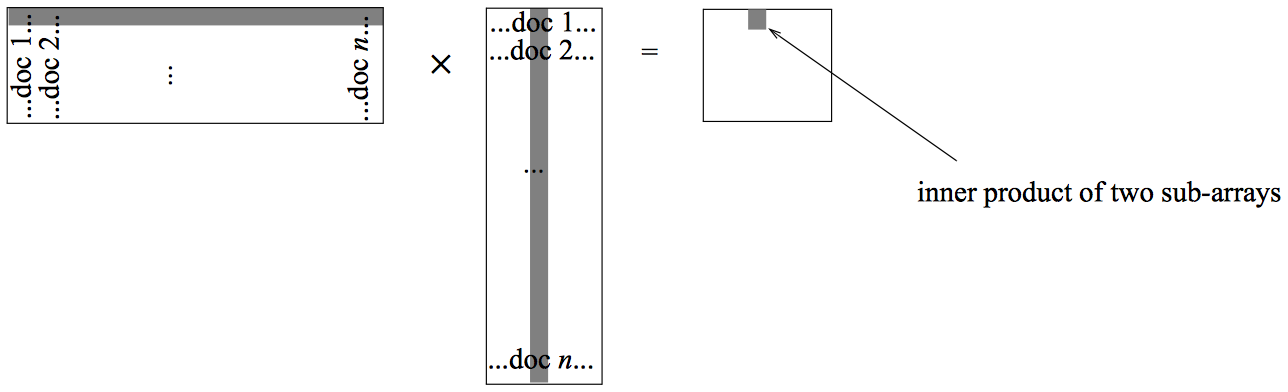
\includegraphics[width=0.75\textwidth]{coOccur.png}
%
%\begin{noindentitemize}
%\item Pure vector-based
%\item Note that after matrix multiply...
%	\begin{noindentitemize2}
%	\item Entry at pos $(i, j)$ is inner product of row $i$ from LHS, col $j$ from RHS
%	\item So if row $i$ is number of occurs of word $i$ in every doc
%	\item And if col $j$ is number of occurs of word $j$ in every doc	
%	\item Entry at pos $(i, j)$ is number of co-occurs of words $i, j$
%	\item Suggests a super-efficient algorithm
%	\end{noindentitemize2}
%\end{noindentitemize}
%\end{frame}
%
%%***********************************************************
%\begin{frame}{Implementation Three (cont)}
%
%\begin{noindentitemize}
%\item Some useful routines:
%	\begin{noindentitemize2}
%        \item $\texttt{np.transpose (array)}$ computes transpose of matrix in array
%        \item $\texttt{np.dot (array1, array2)}$ computes dot product of 1-d arrays, matrix
%multiply of 2-d
%        \end{noindentitemize2}
%\end{noindentitemize}
%\end{frame}
%
%%***********************************************************
%\begin{frame}{These Three Implementations: The Next Activity}
%
%\begin{noindentitemize}
%\item Compare the three different implementations
%        \begin{noindentitemize2}
%        \item $\texttt{./lectPython/CoOccur.html}$
%        \end{noindentitemize2}
%\end{noindentitemize}
%\end{frame}
%
%%***********************************************************
%

%***********************************************************
%***********************************************************

\begin{frame}{Wrap up}
\begin{enumerate}
\item Python review
\item Introduction to numpy
\end{enumerate}

\begin{itemize}
	\item[?] How can we use what we learned today?
	\vspace{2em}
	\item[?] What do we know now that we didn't know before?
\end{itemize}


\end{frame}






\end{document}
